\documentclass[11pt]{article}
\usepackage{amsmath,amsbsy,amssymb,verbatim,fullpage,ifthen,graphicx,bm,amsfonts,amsthm,url}
\usepackage{graphicx}
\usepackage{xcolor}
\usepackage{listings}
\newcommand{\mfile}[1]  {{\small \verbatiminput{./#1}}} % Jeff Fessler, input matlab file
\newcommand{\tmop}[1]{\ensuremath{\operatorname{#1}}}
%\newcommand*{\qed}{\hfill\ensuremath{\blacksquare}}%
\newcommand{\R}{\mathbb{R}}
\newcommand{\C}{\mathbb{C}}
\newcommand{\Z}{\mathbb{Z}}
\newcommand{\A}{\mathcal{A}}
\newcommand{\minimize}{\operatorname*{minimize\ }}
\newcommand{\maximize}{\operatorname*{maximize}}
\newcommand{\opdet}[1]{\operatorname{\textbf{det}}\left(#1\right)}
\newcommand{\optr}[1]{\operatorname{\textbf{tr}}\left(#1\right)}
%\newcommand{\AnswerDefine}{}
\newcommand{\answer}[2][blue]{\ifdefined\AnswerDefine{\color{#1}\it#2}\fi}
\newcommand{\mtx}[1]{\mathbf{#1}}
\newcommand{\vct}[1]{\mathbf{#1}}
\def \lg       {\langle}
\def \rg       {\rangle}
\def \mA {\mtx{A}}
\def \mF {\mtx{F}}
\def \mG {\mtx{G}}
\def \mI {\mtx{I}}
\def \mJ {\mtx{J}}
\def \mU {\mtx{U}}
\def \mS {\mtx{S}}
\def \mV {\mtx{V}}
\def \mW {\mtx{W}}
\def \mLambda {\mtx{\Lambda}}
\def \mSigma {\mtx{\Sigma}}
\def \mX {\mtx{X}}
\def \mY {\mtx{Y}}
\def \mZ {\mtx{Z}}
\def \zero     {\mathbf{0}}
\def \vzero    {\vct{0}}
\def \vone    {\vct{1}}
\def \va {\vct{a}}
\def \vg {\vct{g}}
\def \vu {\vct{u}}
\def \vv {\vct{v}}
\def \vw {\vct{w}}
\def \vx {\vct{x}}
\def \vy {\vct{y}}
\def \vz {\vct{z}}
\def \vphi {\vct{\phi}}
\def \vmu {\vct{\mu}}
\def \R {\mathbb{R}}

%\newcommand{\st}{\operatorname*{\ subject\ to\ }}
\usepackage{algorithm,algpseudocode}
\usepackage{xspace}
% Add a period to the end of an abbreviation unless there's one
% already, then \xspace.
\makeatletter
\DeclareRobustCommand\onedot{\futurelet\@let@token\@onedot}
\def\@onedot{\ifx\@let@token.\else.\null\fi\xspace}

\def\eg{\emph{e.g}\onedot} \def\Eg{\emph{E.g}\onedot}
\def\ie{\emph{i.e}\onedot} \def\Ie{\emph{I.e}\onedot}
\def\cf{\emph{c.f}\onedot} \def\Cf{\emph{C.f}\onedot}
\def\etc{\emph{etc}\onedot} \def\vs{\emph{vs}\onedot}
\def\wrt{w.r.t\onedot} \def\dof{d.o.f\onedot}
\def\etal{\emph{et al}\onedot} \def\st{\emph{s.t}\onedot}
\pagestyle{plain}

\title{{\bf Homework Set 5, CPSC 8420, Fall 2024}} % Change to the appropriate homework number
\author{\Large\underline{Collins, Matthew}}
\date{\textbf{\Large\textcolor{red}{Due 11/27/2024, 11:59PM EST}}} % put your name in the LastName, FirstName format
%\date{\today}

\begin{document}
\maketitle
\section*{Problem 1}
Recall the classification models we discussed in class: \textbf{SVM} and \textbf{Logistic Regression}, seems both of them work on binary classification task. However, in real-world applications, multi-classification is everywhere, thus in this problem we explore how to extend vanilla \textbf{Logistic Regression} for multi-classification. Assume we have $K$ different classes and the input $
\vx\in\mathcal{R}^d$, and the probability to each class is defined as:
\begin{equation}
	\begin{aligned}
		&P(Y=k|X=\vx) =  \frac{exp(\vw_k^T\vx)}{ 1+\sum_{l=1}^{K-1}exp(\vw_l^T\vx)} \quad for  \quad k=1,2,\dots,K-1;\\&P(Y=K|X=\vx) =  \frac{1} { 1+\sum_{l=1}^{K-1}exp(\vw_l^T\vx)}
	\end{aligned}
\end{equation}
If we define $\vw_K=\vzero$, then we can combine the two cases above as one:
\begin{equation}
	P(Y=k|X=\vx) =  \frac{exp(\vw_k^T\vx)}{ 1+\sum_{l=1}^{K-1}exp(\vw_l^T\vx)} \quad for  \quad k=1,\dots,K
\end{equation}
\begin{enumerate}
	\item What and how many parameters are there to be optimized? 

	\item The training data is given as: $\{(\vx_1,y_1),\dots,(\vx_n,y_n)\}$, please simplify the log likelihood function to your best:
	\begin{equation}\label{ori}
		L(\vw_1,\dots,\vw_{K-1})=\sum\limits_{i=1}^n ln P(Y=y_i|X=\vx_i)
	\end{equation}
	\item Now please find the gradient of $L$ \wrt $\vw_k$.
	\item If we add regularization term and formulate new objective function as:
	\begin{equation}\label{reg}
		f(\vw_1,\dots,\vw_{K-1})=L(\vw_1,\dots,\vw_{K-1})-\frac{\lambda}{2}\sum\limits_{l=1}^{K-1}\|\vw_l\|^2_2,
	\end{equation}
	now please determine the new gradient.
	\item You are given \textit{USPS} handwritten recognition digit dataset, with image size $16 \times 16$. For each digit (\ie 0,1,\dots,9) there are 600 training samples in addition to 500 testing ones. You may use: imshow(reshape($\vx$,16,16)) to view the image in Matlab. (Non-Matlab user may utilize .txt files to conduct experiments.)
	\begin{enumerate}
		\item Please use gradient ascent algorithm (you are expected to complete log\_grad.m) to train the model and plot 1) vanilla objective function L in Eq.(\ref{ori}); 2) training accuracy and 3) testing accuracy with updates respectively. Also indicate the final testing accuracy score. (Please choose a proper learning rate and stopping criterion). The folder include figures for your reference. 
		\item Now if we add the regularization term as Eq.(\ref{reg}), please show the final accuracy when $\lambda=\{0,1,10,100,200\}$ respectively.
		\item What conclusion can we draw from the above experiments?
	\end{enumerate}
\end{enumerate}
\textcolor{red}{P1.1, Answer:}\\

For the given multi-class logistic regression model, the parameters to be optimized are the weight vectors 
\( \{\mathbf{w}_1, \mathbf{w}_2, \dots, \mathbf{w}_{K-1}\} \), where each \( \mathbf{w}_k \in \mathbb{R}^d \) is a \( d \)-dimensional 
vector corresponding to one of the \( K-1 \) classes. The parameter \( \mathbf{w}_K \) is fixed to \( \mathbf{0} \), 
so it does not need to be optimized. As a result, the total number of parameters to estimate is given by \( (K-1) \times d \), 
where \( K-1 \) represents the number of weight vectors to optimize, and \( d \) is the number of features in the input \( \mathbf{x} \). 
These parameters are learned during the training process to maximize the likelihood of the observed data.\\

\textcolor{red}{P1.2, Answer:}\\

Using the probability definition from the model, for \( y_i = k \), where \( k \in \{1, \dots, K-1\} \), the conditional probability is given by:
\[
P(Y = k | X = \mathbf{x}_i) = \frac{\exp(\mathbf{w}_k^\top \mathbf{x}_i)}{1 + \sum_{l=1}^{K-1} \exp(\mathbf{w}_l^\top \mathbf{x}_i)}.
\]
For \( y_i = K \), the conditional probability is:
\[
P(Y = K | X = \mathbf{x}_i) = \frac{1}{1 + \sum_{l=1}^{K-1} \exp(\mathbf{w}_l^\top \mathbf{x}_i)}.
\]

The log-likelihood can then be expressed as:
\[
L(\mathbf{w}_1, \dots, \mathbf{w}_{K-1}) = \sum_{i=1}^n \ln P(Y = y_i | X = \mathbf{x}_i).
\]

Substituting the expressions for \( P(Y = y_i | X = \mathbf{x}_i) \):
\[
L(\mathbf{w}_1, \dots, \mathbf{w}_{K-1}) = \sum_{i=1}^n \left[ \mathbf{I}_{\{y_i < K\}} \ln \left( \frac{\exp(\mathbf{w}_{y_i}^\top \mathbf{x}_i)}{1 + \sum_{l=1}^{K-1} \exp(\mathbf{w}_l^\top \mathbf{x}_i)} \right) + \mathbf{1}_{\{y_i = K\}} \ln \left( \frac{1}{1 + \sum_{l=1}^{K-1} \exp(\mathbf{w}_l^\top \mathbf{x}_i)} \right) \right],
\]
where \( \mathbf{1}_{\{y_i < K\}} \) is the indicator function that is 1 if \( y_i \in \{1, \dots, K-1\} \), and \( \mathbf{1}_{\{y_i = K\}} \) is 1 if \( y_i = K \).

For \( y_i < K \), the first term simplifies to:
\[
\ln \left( \frac{\exp(\mathbf{w}_{y_i}^\top \mathbf{x}_i)}{1 + \sum_{l=1}^{K-1} \exp(\mathbf{w}_l^\top \mathbf{x}_i)} \right) = \mathbf{w}_{y_i}^\top \mathbf{x}_i - \ln \left( 1 + \sum_{l=1}^{K-1} \exp(\mathbf{w}_l^\top \mathbf{x}_i) \right).
\]
For \( y_i = K \), the second term simplifies to:
\[
\ln \left( \frac{1}{1 + \sum_{l=1}^{K-1} \exp(\mathbf{w}_l^\top \mathbf{x}_i)} \right) = - \ln \left( 1 + \sum_{l=1}^{K-1} \exp(\mathbf{w}_l^\top \mathbf{x}_i) \right).
\]

Combining these, the log-likelihood simplifies to:
\[
L(\mathbf{w}_1, \dots, \mathbf{w}_{K-1}) = \sum_{i=1}^n \left[ \mathbf{w}_{y_i}^\top \mathbf{x}_i \mathbf{I}_{\{y_i < K\}} - \ln \left( 1 + \sum_{l=1}^{K-1} \exp(\mathbf{w}_l^\top \mathbf{x}_i) \right) \right].
\]

Here, the first term contributes only when \( y_i < K \), while the second term applies to all data points.




\textcolor{red}{P1.3, Answer:}\\


The first term in the summation contributes only when \( y_i = k \). Therefore:
\[
\frac{\partial}{\partial \mathbf{w}_k} \left( \mathbf{w}_{y_i}^\top \mathbf{x}_i \right) = 
\begin{cases}
\mathbf{x}_i & \text{if } y_i = k, \\
0 & \text{if } y_i \neq k.
\end{cases}
\]

The second term is the log of the denominator:
\[
\frac{\partial}{\partial \mathbf{w}_k} \ln \left( 1 + \sum_{l=1}^{K-1} \exp(\mathbf{w}_l^\top \mathbf{x}_i) \right).
\]
Let:
\[
f(\mathbf{w}_k) = \ln \left( 1 + \sum_{l=1}^{K-1} \exp(\mathbf{w}_l^\top \mathbf{x}_i) \right).
\]
The derivative of \( f \) with respect to \( \mathbf{w}_k \) is:
\[
\frac{\partial f}{\partial \mathbf{w}_k} = \frac{\exp(\mathbf{w}_k^\top \mathbf{x}_i) \mathbf{x}_i}{1 + \sum_{l=1}^{K-1} \exp(\mathbf{w}_l^\top \mathbf{x}_i)}.
\]

Combining these, the gradient of \( L \) with respect to \( \mathbf{w}_k \) is:
\[
\frac{\partial L}{\partial \mathbf{w}_k} = \sum_{i=1}^n \left[ \mathbf{I}_{\{y_i = k\}} \mathbf{x}_i - \frac{\exp(\mathbf{w}_k^\top \mathbf{x}_i) \mathbf{x}_i}{1 + \sum_{l=1}^{K-1} \exp(\mathbf{w}_l^\top \mathbf{x}_i)} \right],
\]
where \( \mathbf{1}_{\{y_i = k\}} \) is the indicator function that equals 1 if \( y_i = k \), and 0 otherwise.

Simplifying further, let:
\[
P(Y = k | \mathbf{x}_i) = \frac{\exp(\mathbf{w}_k^\top \mathbf{x}_i)}{1 + \sum_{l=1}^{K-1} \exp(\mathbf{w}_l^\top \mathbf{x}_i)}.
\]
Then the gradient can be written as:
\[
\frac{\partial L}{\partial \mathbf{w}_k} = \sum_{i=1}^n \mathbf{x}_i \left[ \mathbf{I}_{\{y_i = k\}} - P(Y = k | \mathbf{x}_i) \right].
\]

This is the gradient of the log-likelihood \( L \) with respect to \( \mathbf{w}_k \). It consists of the difference between the observed indicator for class \( k \) and the predicted probability for class \( k \), scaled by the feature vector \( \mathbf{x}_i \).


\textcolor{red}{P1.4, Answer:}\\

To determine the gradient of the regularized objective function, we begin with the definition of \( f \), which is given by:
\[
f(\mathbf{w}_1, \dots, \mathbf{w}_{K-1}) = L(\mathbf{w}_1, \dots, \mathbf{w}_{K-1}) - \frac{\lambda}{2} \sum_{l=1}^{K-1} \|\mathbf{w}_l\|_2^2,
\]
where \( L(\mathbf{w}_1, \dots, \mathbf{w}_{K-1}) \) is the log-likelihood function:
\[
L(\mathbf{w}_1, \dots, \mathbf{w}_{K-1}) = \sum_{i=1}^n \left[ \mathbf{w}_{y_i}^\top \mathbf{x}_i - \ln \left( 1 + \sum_{l=1}^{K-1} \exp(\mathbf{w}_l^\top \mathbf{x}_i) \right) \right].
\]

To compute the gradient of \( f \) with respect to \( \mathbf{w}_k \), we compute the derivative of each term in \( f \). First, the gradient of \( L \) with respect to \( \mathbf{w}_k \) is:
\[
\nabla L(\mathbf{w}_k) = \sum_{i=1}^n \mathbf{x}_i \left[ I(y_i = k) - P(Y = k | X = \mathbf{x}_i) \right],
\]
where \( P(Y = k | X = \mathbf{x}_i) = \frac{\exp(\mathbf{w}_k^\top \mathbf{x}_i)}{1 + \sum_{l=1}^{K-1} \exp(\mathbf{w}_l^\top \mathbf{x}_i)} \), and \( I(y_i = k) \) is the indicator function that equals 1 if \( y_i = k \), and 0 otherwise.

The gradient of the regularization term \( -\frac{\lambda}{2} \sum_{l=1}^{K-1} \|\mathbf{w}_l\|_2^2 \) with respect to \( \mathbf{w}_k \) is:
\[
\nabla \left( -\frac{\lambda}{2} \sum_{l=1}^{K-1} \|\mathbf{w}_l\|_2^2 \right) = -\lambda \mathbf{w}_k.
\]

Combining these results, the gradient of \( f \) with respect to \( \mathbf{w}_k \) is:
\[
\nabla f(\mathbf{w}_k) = \nabla L(\mathbf{w}_k) - \lambda \mathbf{w}_k.
\]

Substituting the expression for \( \nabla L(\mathbf{w}_k) \):
\[
\nabla f(\mathbf{w}_k) = \sum_{i=1}^n \mathbf{x}_i \left[ I(y_i = k) - P(Y = k | X = \mathbf{x}_i) \right] - \lambda \mathbf{w}_k.
\]


\textcolor{red}{P1.5.a, Answer:}\\

For the Matlab code in 1.5.a, I used a stepsize of 0.0001 and iterations of 5000.
For lambda = 0, I graphed my objective value, training accuracy, and testing accuracy v.s. iterations. 
The results can be seen in Figures 1, 2, and 3. The final accuracy for lambda = 0 can be seen in Figure 4.\\

\begin{figure}[h]
    \centering
    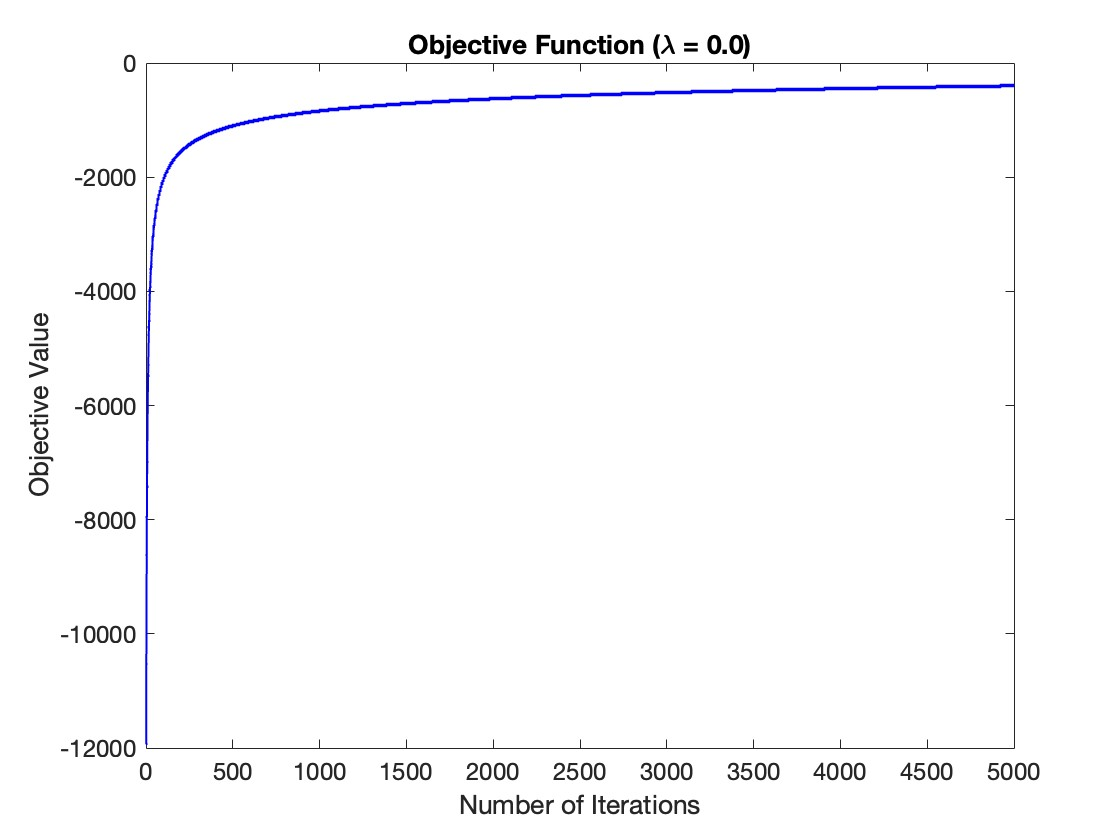
\includegraphics[width=0.95\linewidth]{objective_lambda_0.0.jpg}
    \caption{Objective Value}
    \label{fig:objective}
\end{figure}


\begin{figure}[h]
    \centering
    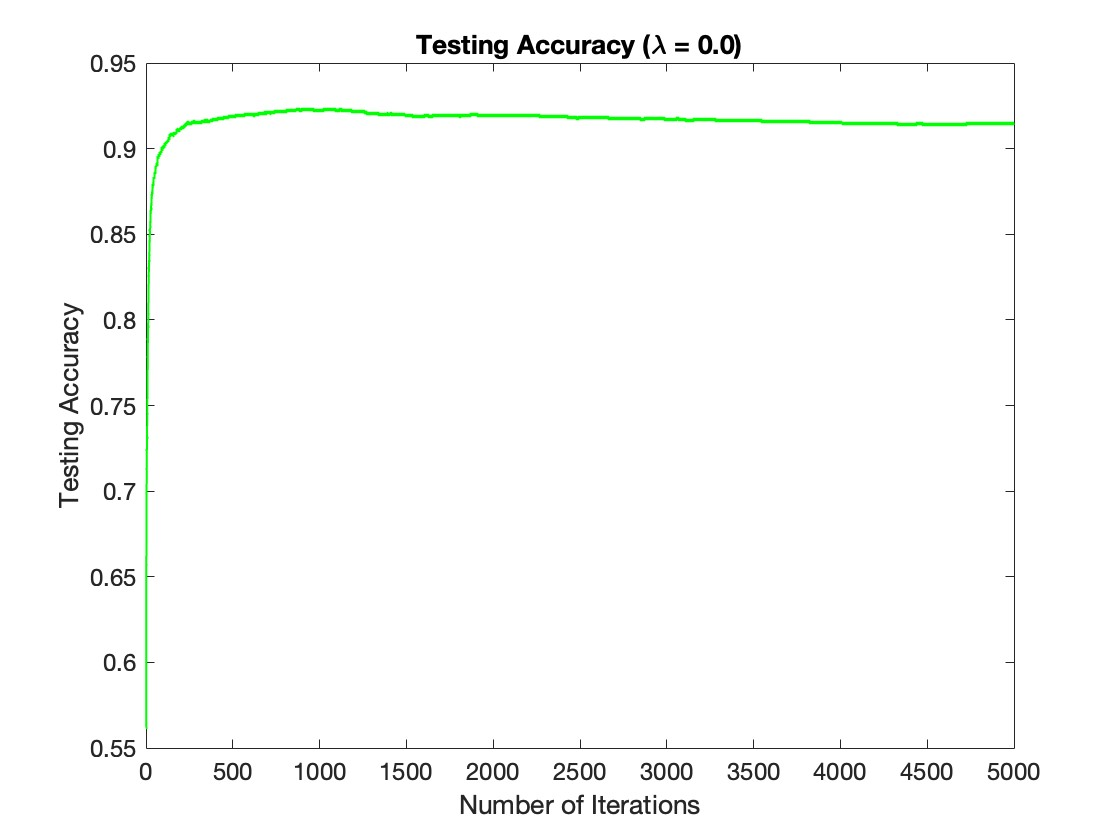
\includegraphics[width=0.95\linewidth]{test_accuracy_lambda_0.0.jpg}
    \caption{Test Accuracy}
    \label{fig:test}
\end{figure}


\begin{figure}[h]
    \centering
    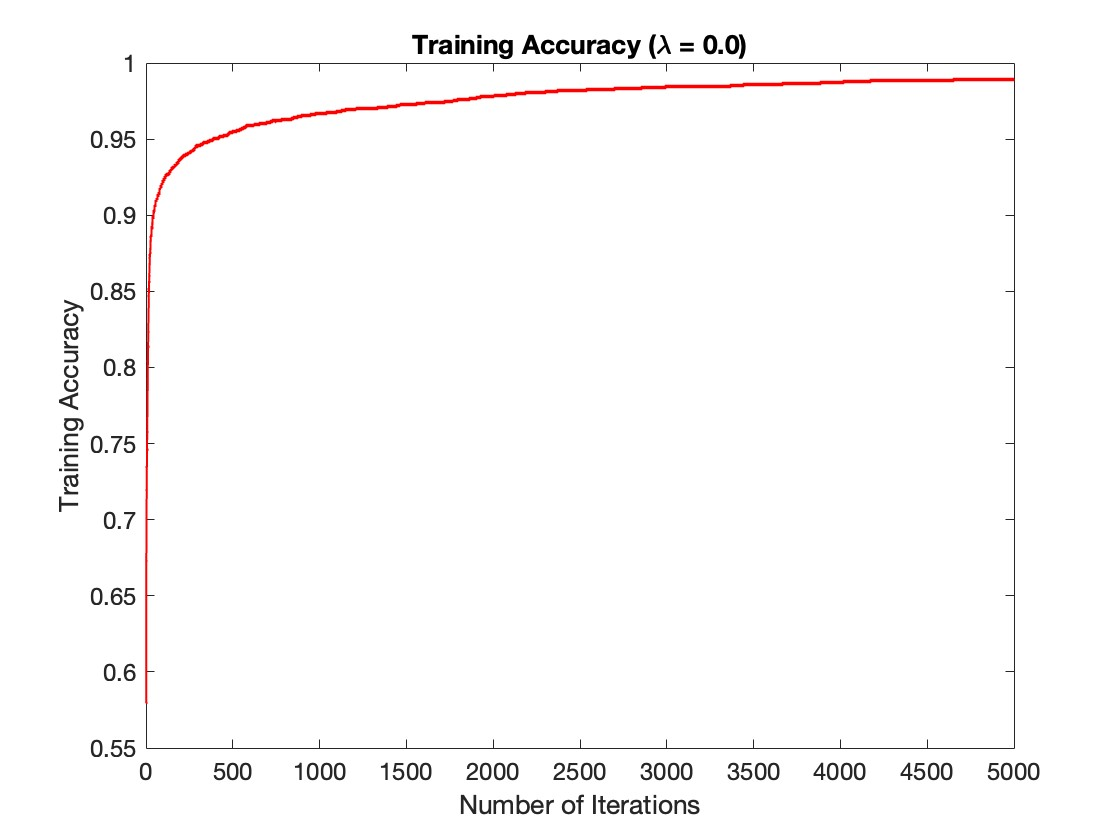
\includegraphics[width=0.95\linewidth]{train_accuracy_lambda_0.0.jpg}
    \caption{Train Accuracy}
    \label{fig:train}
\end{figure}

\begin{figure}[h]
    \centering
    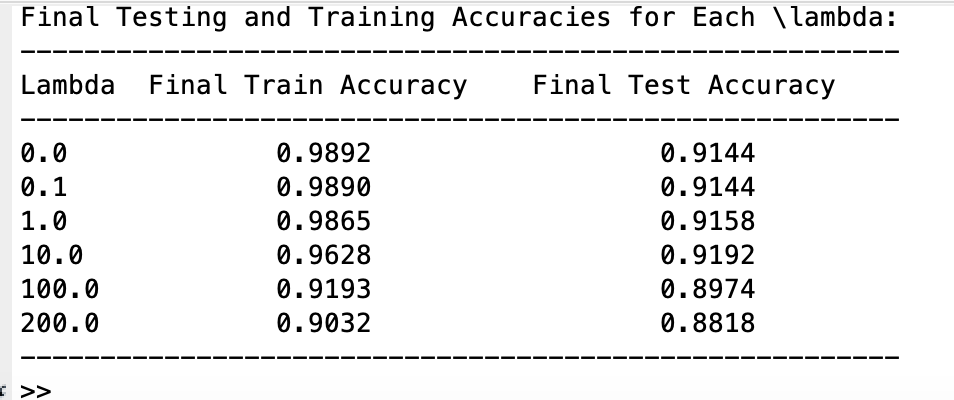
\includegraphics[width=0.95\linewidth]{final_accuracy.png}
    \caption{Final Accuracy}
    \label{fig:final}
\end{figure}


\textcolor{red}{P1.5.b, Answer:}\\

The final accuracy for the given lambdas can be seen in Figure 4.\\

\textcolor{red}{P1.5.c, Answer:}\\

From the results of the experiments, we observe that adding a regularization term can help avoid overfitting and improve 
generalization performance. For example, with a moderate regularization parameter such as \( \lambda = 10 \), 
the model achieves better performance on the testing set while maintaining high accuracy on the training set. 
This indicates that regularization helps control the complexity of the model, preventing it from memorizing the training 
data and instead promoting generalization to unseen data. However, it is also evident that the regularization parameter cannot 
be too large. Excessive regularization, as seen with higher values of \( \lambda \) (e.g., \( \lambda = 100 \) or \( \lambda = 200 \)), 
overly constrains the model, leading to underfitting and a decrease in both training and testing accuracy. 
Therefore, an optimal balance in the choice of \( \lambda \) is crucial to achieve the best generalization performance.
\clearpage

\appendix

\section{Appendix: MATLAB Code}

\begin{lstlisting}[language = matlab]
	function G=log_grad(y, X, B) 

	%compute gradient 
	
		K_1=size(B,2);
		eXB=exp(X*B);
		s_eXB=1./(sum(eXB, 2)+1);
		eXB=eXB.*repmat(s_eXB, 1, K_1);
		
		for k= 1: K_1
			eXB(:,k)=(y==k)-eXB(:,k);
		end
		
		G=(X'*eXB);
	
	end
\end{lstlisting}

\begin{lstlisting}[language = matlab]
	clear; clc; close all;

	load usps_digital.mat;
	
	learning_rate = 1e-4;   
	max_iterations = 5000;  
	lambdas = [0, 0.1, 1, 10, 100, 200]; 
	
	final_test_accuracies = zeros(size(lambdas));
	final_train_accuracies = zeros(size(lambdas));
	
	for idx = 1:length(lambdas)
		lambda = lambdas(idx); 
		
		[B, test_error, train_error, objective_values] = log_reg(tr_y, tr_X, te_y, te_X, lambda, learning_rate);
		
		final_test_accuracies(idx) = test_error(end);
		final_train_accuracies(idx) = train_error(end);
		
		figure;
		plot(1:length(objective_values)-1, objective_values(1:end-1), 'b-o', 'LineWidth', 1, 'MarkerSize', 1);
		title(sprintf('Objective Function (\\lambda = %.1f)', lambda), 'FontSize', 15);
		xlabel('Number of Iterations', 'FontSize', 15);
		ylabel('Objective Value', 'FontSize', 15);
		set(gca, 'FontSize', 12);
		saveas(gcf, sprintf('objective_lambda_%.1f.fig', lambda));
		
		figure;
		plot(1:length(train_error)-1, train_error(1:end-1), 'r-o', 'LineWidth', 1, 'MarkerSize', 1);
		title(sprintf('Training Accuracy (\\lambda = %.1f)', lambda), 'FontSize', 15);
		xlabel('Number of Iterations', 'FontSize', 15);
		ylabel('Training Accuracy', 'FontSize', 15);
		set(gca, 'FontSize', 12);
		saveas(gcf, sprintf('train_accuracy_lambda_%.1f.fig', lambda));
		
		figure;
		plot(1:length(test_error)-1, test_error(1:end-1), 'g-o', 'LineWidth', 1, 'MarkerSize', 1);
		title(sprintf('Testing Accuracy (\\lambda = %.1f)', lambda), 'FontSize', 15);
		xlabel('Number of Iterations', 'FontSize', 15);
		ylabel('Testing Accuracy', 'FontSize', 15);
		set(gca, 'FontSize', 12);
		saveas(gcf, sprintf('test_accuracy_lambda_%.1f.fig', lambda));
	end
	
	fprintf('Final Testing and Training Accuracies for Each \\lambda:\n');
	fprintf('-------------------------------------------------------\n');
	fprintf('Lambda\tFinal Train Accuracy\tFinal Test Accuracy\n');
	fprintf('-------------------------------------------------------\n');
	for idx = 1:length(lambdas)
		fprintf('%.1f\t\t%.4f\t\t\t%.4f\n', lambdas(idx), final_train_accuracies(idx), final_test_accuracies(idx));
	end
	fprintf('-------------------------------------------------------\n');
	
	save('final_accuracies.mat', 'lambdas', 'final_train_accuracies', 'final_test_accuracies');
\end{lstlisting}
\end{document}
